\begin{pastexam}[label={px:ust-110-ee-ds-09}]{臺聯大電機類 110 學年度 第 9 題}
（問答）

(10\%) The binary search tree in Figure 2 was created by starting with a null tree and entering data from
the keyboard. In what sequence were the data entered? If there is more than one possible sequence,
identify the alternatives.

\begin{center}
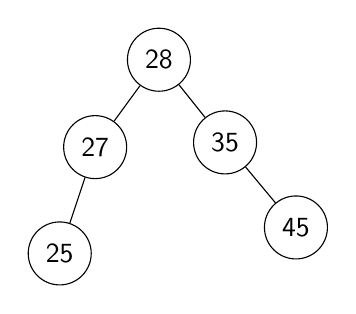
\begin{tikzpicture}[n/.style={circle,draw,fill=white,inner sep=0pt,minimum size=8mm,font=\sffamily}]
\node[n] (n28) at (1.26,0.00) {28};
\node[n] (n27) at (0.45,-1.11) {27};
\node[n] (n35) at (2.10,-1.05) {35};
\node[n] (n25) at (0.00,-2.46) {25};
\node[n] (n45) at (3.00,-2.13) {45};
\draw (n28)--(n27);
\draw (n28)--(n35);
\draw (n27)--(n25);
\draw (n35)--(n45);
\end{tikzpicture}\\[2pt] Figure 2. Binary search tree.\end{center}
\end{pastexam}

\begin{pastsoln}
答案：共 $6$ 種輸入順序：
\begin{center}
\begin{tabular}{ll}
28, 27, 25, 35, 45 & 28, 35, 27, 25, 45 \\
28, 27, 35, 25, 45 & 28, 35, 27, 45, 25 \\
28, 27, 35, 45, 25 & 28, 35, 45, 27, 25
\end{tabular}
\end{center}

二元搜尋樹的插入（資結書第~9.2~節）一定把新鍵接成葉節點，已經在樹裡的節點位置不會再變。 所以一個節點
在樹裡是另一個節點的祖先，就表示它\textbf{比較早}輸入。 反過來，只要每個節點都在它所有祖先之後輸入，插入
時沿路比較的對象就是那些祖先，它一定落在圖上的位置。 因此可能的輸入順序，就是「每個節點都排在它的祖先
後面」的所有排列。

\textbf{條件。}
\begin{itemize}
\item $28$ 是根，是所有節點的祖先，必須第一個輸入。
\item $27$ 是 $25$ 的父節點：$27$ 在 $25$ 前面。
\item $35$ 是 $45$ 的父節點：$35$ 在 $45$ 前面。
\item 左子樹 $\{27, 25\}$ 和右子樹 $\{35, 45\}$ 之間沒有祖先關係，誰先誰後都可以。
\end{itemize}

\textbf{計數。} $28$ 之後的 $4$ 個位置，選 $2$ 個給左子樹（順序固定是 $27, 25$），其餘給右子樹（順序固定
是 $35, 45$）：$\binom{4}{2} = 6$ 種，就是上表。 例如 $28, 35, 27, 45, 25$：$35 > 28$ 接在右邊；
$27 < 28$ 接在左邊；$45 > 28$、$45 > 35$ 接在 $35$ 的右邊；$25 < 28$、$25 < 27$ 接在 $27$ 的左邊，和
圖一樣。 反例：$28, 25, 27, \ldots$ 會讓 $25$ 成為 $28$ 的左子節點、$27$ 接在 $25$ 的右邊，形狀不同。
\end{pastsoln}
